\chapter{MLOF Evaluation in Simulations}\label{C:Evaluation}
In this chapter, we evaluate MLOF with two embedded models, a decision
tree (DT) and a Light Gradient Boosting Machine (LGBM) regressor,
against the Contiki-NG objective functions OF0 and MRHOF. We compare
their QoS in random topologies of 60 to 100 nodes under increasing
traffic load, and then quantify the overhead introduced by MLOF.

\section{Pilot Test of MLOF}
In this section, we run four models on a fast simulation using random
topologies to test the feasibility of each model. We run the test on
60 nodes with varying traffic rate from 64 to 128 for 600 seconds.
Figure~\ref{fig:} shows the PDR of the pilot test.

The results shows that linear regressoin and SVR model suffers in terms of PDR.
Because of this, we remove linear regression and SVR from subsequent
simulations and explain the possible reason for such degraded
performance in the MLOF overhead.

% TODO: include prerun
\section{Simulation Settings}
Table~\ref{tab:sim-parameters} shows the simulation parameters
with the total of 3000 simulations across 25 random topologies and
two different seed to choose the overloading clients, resulting in 50
different runs for each pair of traffic rate and number of nodes. We
then analyse the quality-of-service metrics, the OF resources
consumption in terms
of computation, memory and network overhead, and the produced DODAG
of MLOF and MRHOF.

\begin{table}[h]
    \caption{Simulation parameters for performance evaluation.}
    \label{tab:sim-parameters}
    \begin{center}
        \begin{tabular}{ll}
            \hline
            \textbf{Parameter} & \textbf{Value} \\
            \hline
            Simulator                      & COOJA \\
            Mote type                      & Zolertia Z1 \\
            Simulation Time                & 3600\,s \\
            Number of Nodes                & 60, 80, 100 \\
            Transmission rate              & 90\% \\
            Receiving rate                 & 90\% \\
            Topology                       & Random with seeds 11--35 \\
            MAC Layer Protocol             & CSMA \\
            Radio Range                    & 50\,m \\
            Interference Range             & 60\,m \\
            Packet Size                    & 64 bytes \\
            % TODO: line break here
            Routing Protocol               & \makecell{MLOF\_DTree,
            MLOF\_LGMB, OF0 and MRHOF} \\
            Traffic rate per node          & 64, 80, 96, 112, 128\,bps \\
            Overloading client traffic rate & 256\,bps \\
            Overloading client rate        & 5\% \\
            Overloading client seed        & 1, 2 \\
            \hline
        \end{tabular}
    \end{center}
\end{table}

\section{QoS Evaluation}
% TODO: introduce the metrics
\subsection{Packet Delivery Performance}
Figure~\ref{fig:pdr_all_nodes} shows the average packet delivery
ratio (PDR) across all random
topologies and overloaded-client positions, with 95\% confidence
intervals over 50 runs for each pair of traffic rate and number of
nodes. Under light load, all OFs reach almost 100\% delivery ratio.
As the load increases, \dtree{} achieves a high PDR for
longer than the other OFs, whereas MRHOF yields the lowest PDR in most
configurations. In all cases, the performance of \lgbm{} is worse
compared to \dtree{}.

At 60 nodes, \dtree{} is the only OF that maintains a PDR above 94\%
across all loads,
which is 11.0 and 17.3 percentage points higher than OF0 and MRHOF at
128~bps, respectively.
\lgbm{} closely follows \dtree{} up to 112~bps (96.5\%), but its PDR
then drops sharply by 14.7 percentage points to 81.8\% at 128~bps,
falling to the level of OF0.

\begin{fig}[tbh]
    \begin{center}
        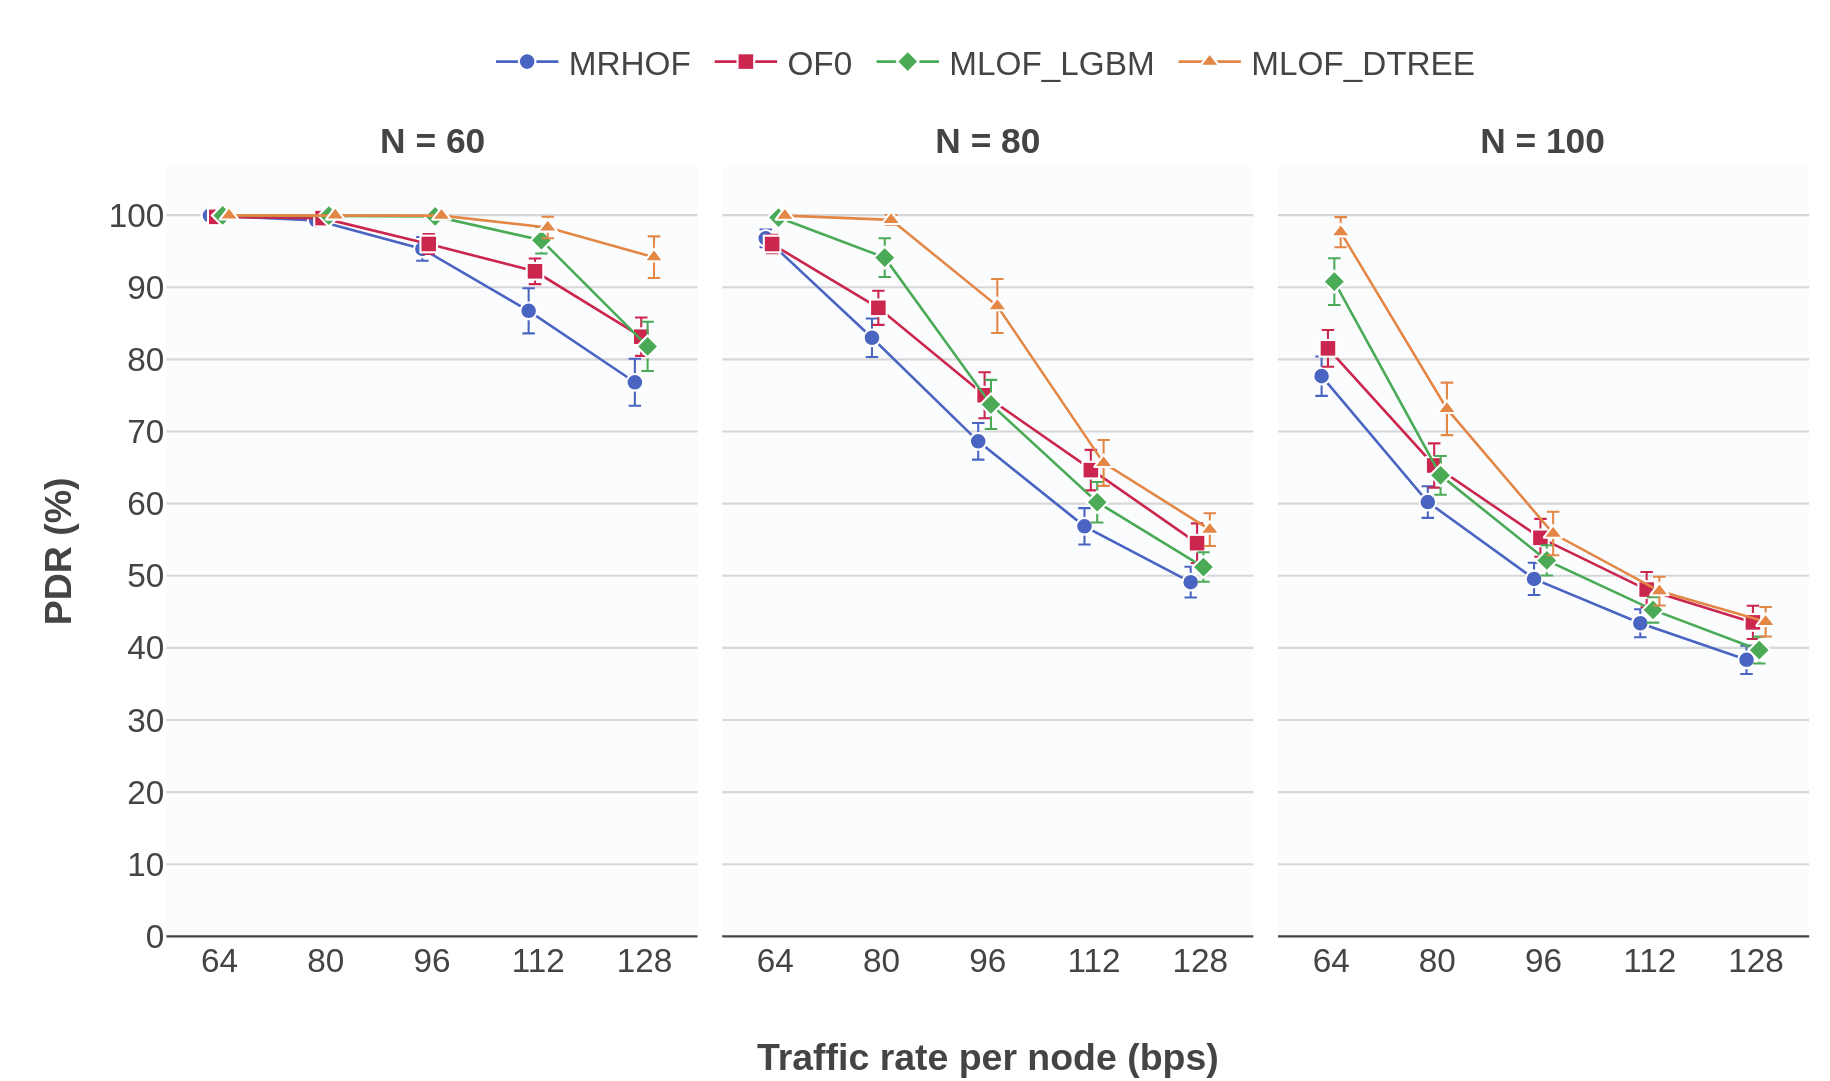
\includegraphics[width=1\textwidth]{assets/pdr_all_nodes.png}
        \caption{Average PDR with 95\% CI for 60, 80 and 100 nodes.}
        \label{fig:pdr_all_nodes}
    \end{center}
\end{fig}

The PDR of \dtree{} plummets as the load increases and the network
grows. At 80 nodes, \dtree{} achieves 87.4\% at 96~bps, which is
12.4 percentage points higher than that of OF0 at 75.0\%. However,
the figure falls to
65.6\% at 112~bps, where its confidence interval overlaps with that
of OF0 at 64.6\%. Likewise, at 100 nodes the largest gap occurs at
64~bps, where \dtree{}
achieves 97.6\% against 81.5\% for OF0, and from 96~bps onward all OFs
except MRHOF perform similarly.
\lgbm{} follows a similar pattern to \dtree{}, outperforming the
standard OFs at light load but degrading rapidly as the load
increases. At 80 nodes it falls from 94.1\% to 73.8\% between 80 and
96~bps, and at 100
nodes from 90.8\% to 63.9\% between 64 and 80~bps, after which it
performs at the level of OF0 or slightly below.
% TODO: elaborate more
One possible reason
for the sharp decrease in PDR is the overhead of \dtree{} and
\lgbm{} becomes more pronounced as the load increases.

\subsection{Latency and Hop Count}
The end-to-end latency is calculated as the difference between the
time the server receives a packet and the time the client sends it:
\begin{equation}
    \text{Latency} = \text{Server receive time} - \text{Client send
    time}
\end{equation}

Figure~\ref{fig:latency_all_nodes} depicts the average end-to-end latency and
Figure~\ref{fig:hop_count_all_nodes} depicts the average hop count.
As shown in these two figures, the average end-to-end latency
closely follows the same trend as the average hop count.
\dtree{} produces the lowest hop count in all configurations, which
corresponds to the lowest latency. For example, at 60 nodes and
128~bps, \dtree{} forms paths of 3.12 hops on average,
compared with 3.89 for OF0 and 4.19 for
MRHOF, resulting in latency of 0.192~s, 0.303~s
and 0.329~s, respectively.
The relationship is further illustrated by MRHOF and OF0. At light
load, MRHOF forms shorter paths and achieves lower latency than OF0,
but its hop count grows faster as the load increases and eventually
overtakes that of OF0, at which point its latency also exceeds that
of OF0.

The correlation between latency and hop count is not linear.
At 100 nodes, the average hop count of \dtree{} increases by 49\%,
from 3.62 to 5.40, between 64 and 128~bps, while its latency more than
triples, from 0.195 to 0.598~s. Thus the longer paths are one part of
the increase in latency. In a more congested network, more
retransmissions are needed per hop, and packets may also spend more
time waiting in queues and in CSMA
backoff to avoid collisions.

\begin{fig}[tbh]
    \begin{center}
        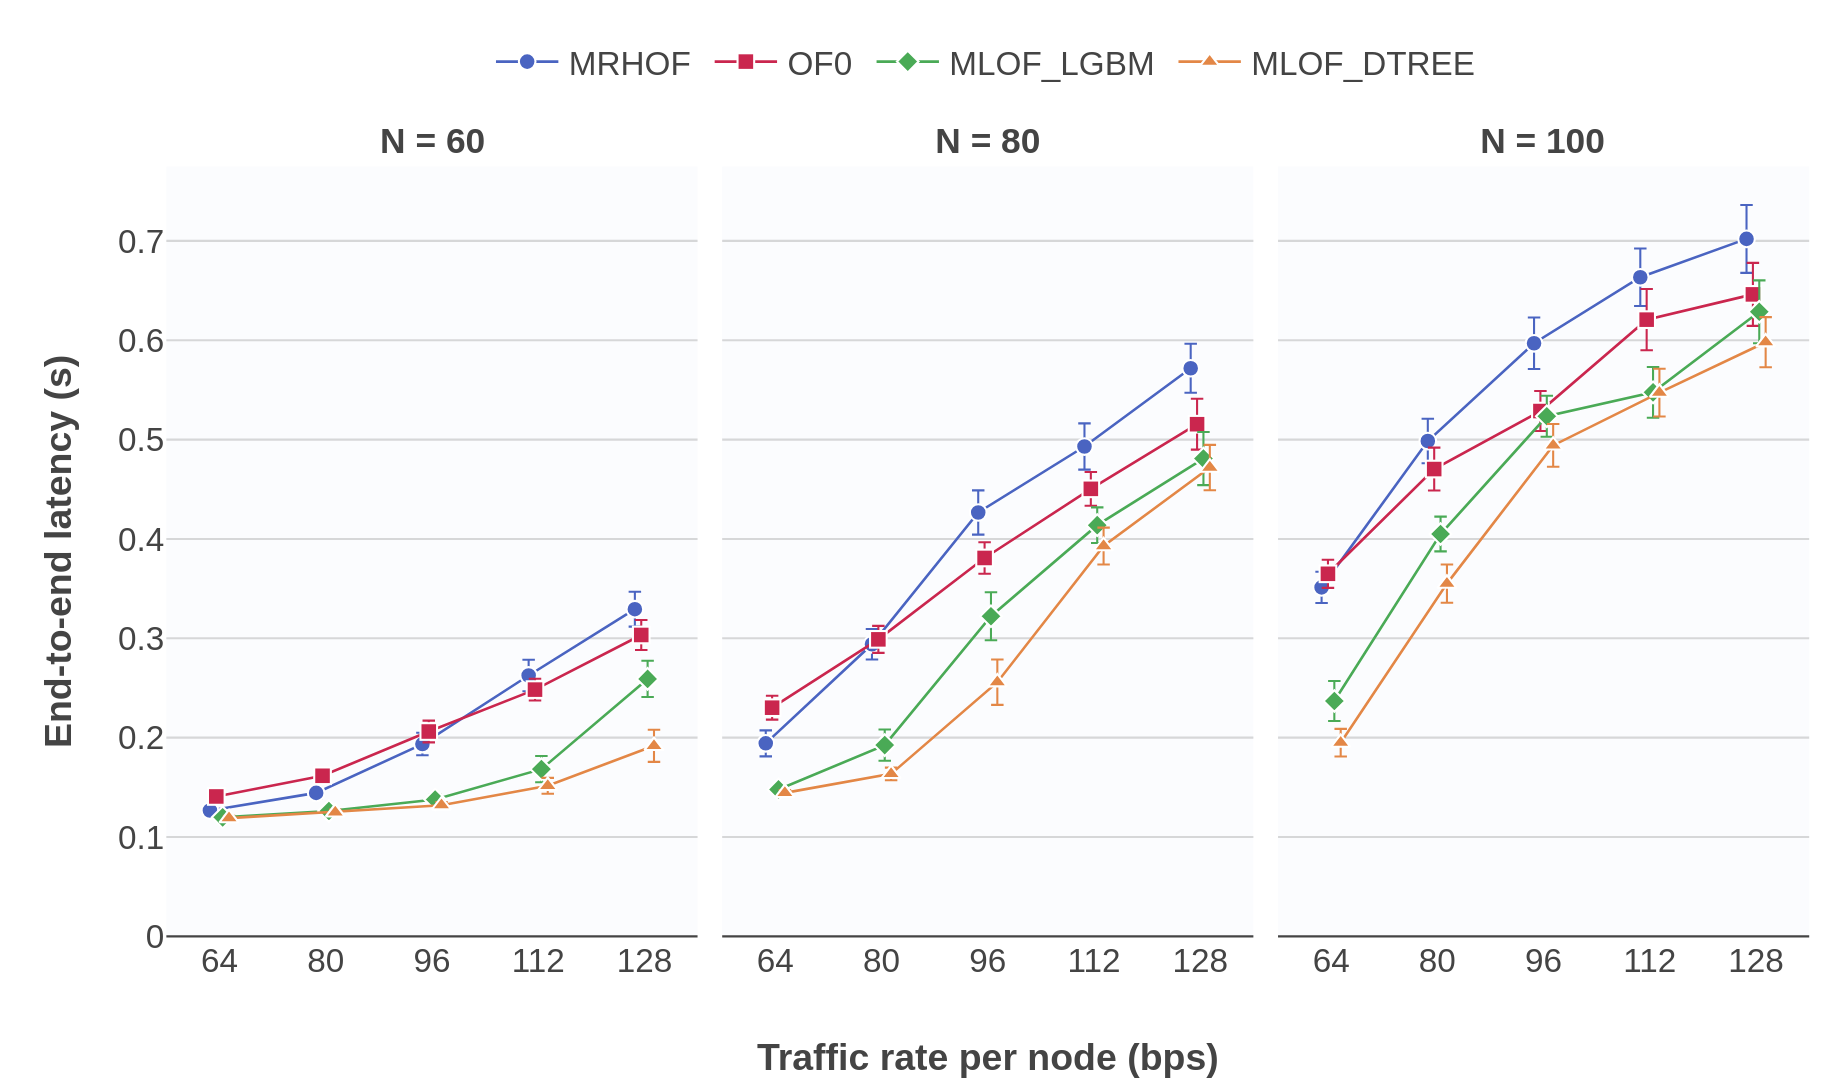
\includegraphics[width=1\textwidth]{assets/latency_all_nodes.png}
        \caption{Average end-to-end latency with 95\% CI for 60, 80
        and 100 nodes.}
        \label{fig:latency_all_nodes}
    \end{center}
\end{fig}

\begin{fig}[tbh]
    \begin{center}

        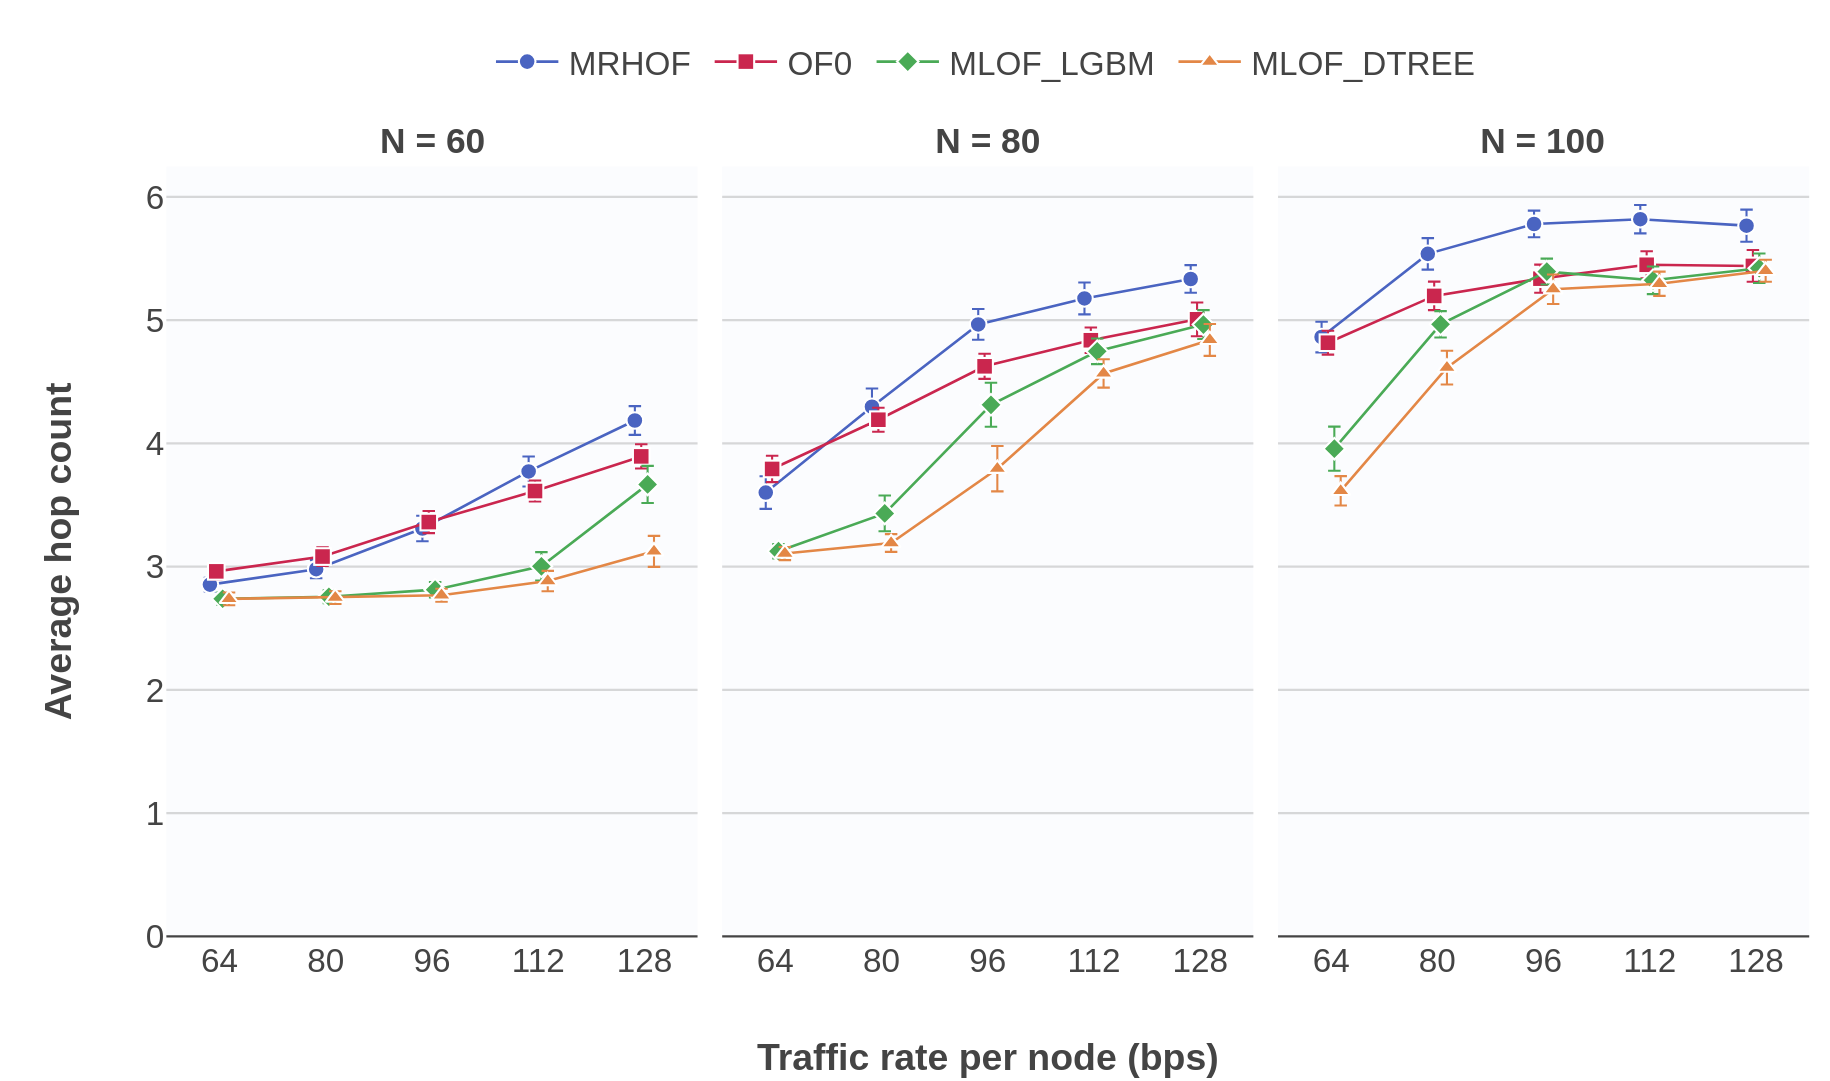
\includegraphics[width=1\textwidth]{assets/hop_count_all_nodes.png}
        \caption{Average hop count with 95\% CI for 60, 80 and 100 nodes.}
        \label{fig:hop_count_all_nodes}
    \end{center}
\end{fig}

The explanation for the low average hop count in OF0 and MLOF of
both models is that both OF0 and MLOF include hop
count in their rank calculation. OF0 does so implicitly by deriving
per-hop step from the link ETX in its rank
increases, whereas MLOF
includes the hop count explicitly as an input feature of the model.
MRHOF considers only the path ETX and may select longer routes when
links become congested.
% TODO: why is hop count of dtree is lower than lgbm

On the other hand, the latency results should be interpreted together with the
PDR as latency is only measured for successfully delivered packets. When
the delivery ratio is low, packets from nodes far from the root, which
would have the highest latency, are more likely to be
dropped and are excluded from the measurement. Thus a reduction
in latency reflects a genuine improvement only when the PDR is maintained or
improved. From this perspective, the lower latency of \lgbm{}
compared with OF0 at high loads should be
interpreted with caution, as \lgbm{} also delivers fewer packets. For
example, at 100 nodes and 112~bps, \lgbm{} achieves a latency of
0.548~s compared with 0.621~s for OF0, but a PDR of only 45.3\%
compared with 48.1\%.

\subsection{CPU Usage and DODAG Stability}
The CPU usage is calculated from the measurement of Energest module
in Contiki-NG
\begin{equation}
    \text{CPU usage (\%)} = \frac{\text{CPU active ticks}}{\text{Total
    ticks}} \times 100
\end{equation}
where the total ticks are the sum of the ticks spent in active mode
and in low-power modes.
For stability, we use the number of parent switches per node and the
average number of DIOs sent per minute per node to measure how stable
the OFs are.
The CPU usage is interpreted together with the routing control traffic
and the forwarding load, since processing DIOs, recomputing ranks and
relaying packets all contribute to it.

Figure~\ref{fig:cpu_all_nodes} shows the average CPU usage, while
Figures~\ref{fig:dio_sent_all_nodes}
and~\ref{fig:parent_switch_all_nodes} show the average number of DIO
messages sent per node per minute and
the average number of parent switches per node, respectively.

At light load, OF0 has the highest CPU usage, e.g.\ 2.73\% at
60 nodes and 64~bps compared with 1.99\% for MRHOF. This aligns
with its unstable parent selection at 102 parent switches
per node and higher DIO transmissions at 5.1 DIOs per minute, against
2.6 parent switches and 1.6 DIOs per minute per node for MRHOF.
The high number of parent switches of OF0 in low traffic can be
attributed to the
fact that OF0 does not employ rank hysteresis, thus minor
fluctuations cause frequent switching. MRHOF and MLOF avoid this by
switching parent only
when the rank improvement exceeds a threshold.

However, the switching rate of MRHOF surges as the load increases, and
reaches or surpasses that of OF0 at 128\,bps for 60, 96\,bps for 80
and 80\,bps for 100 nodes.
Under such heavy load, ETX degrades rapidly because more
retransmissions are needed. The higher number of parent switches
also increases DIO transmissions, since each switch resets the
Trickle timer so the node can quickly propagate the updated
routing information. Together, these effects raise MRHOF's CPU
usage under these conditions.

The switching rate of MLOF
grows considerably more slowly and remains less than half that of both
baselines in all configurations. \dtree{} has the most stable topology up
to moderate loads, e.g.\ 26.2 switches per node at 60 nodes and 128~bps
compared with 55.0 for \lgbm{}. Once the network saturates, at 80 nodes
from 112~bps and at 100 nodes from 80~bps, \lgbm{} switches less often
than \dtree{}. This suggests that the predictions of the single decision tree
become less stable than those of the ensemble when all paths are
congested.
\begin{fig}[tbh]
    \begin{center}
        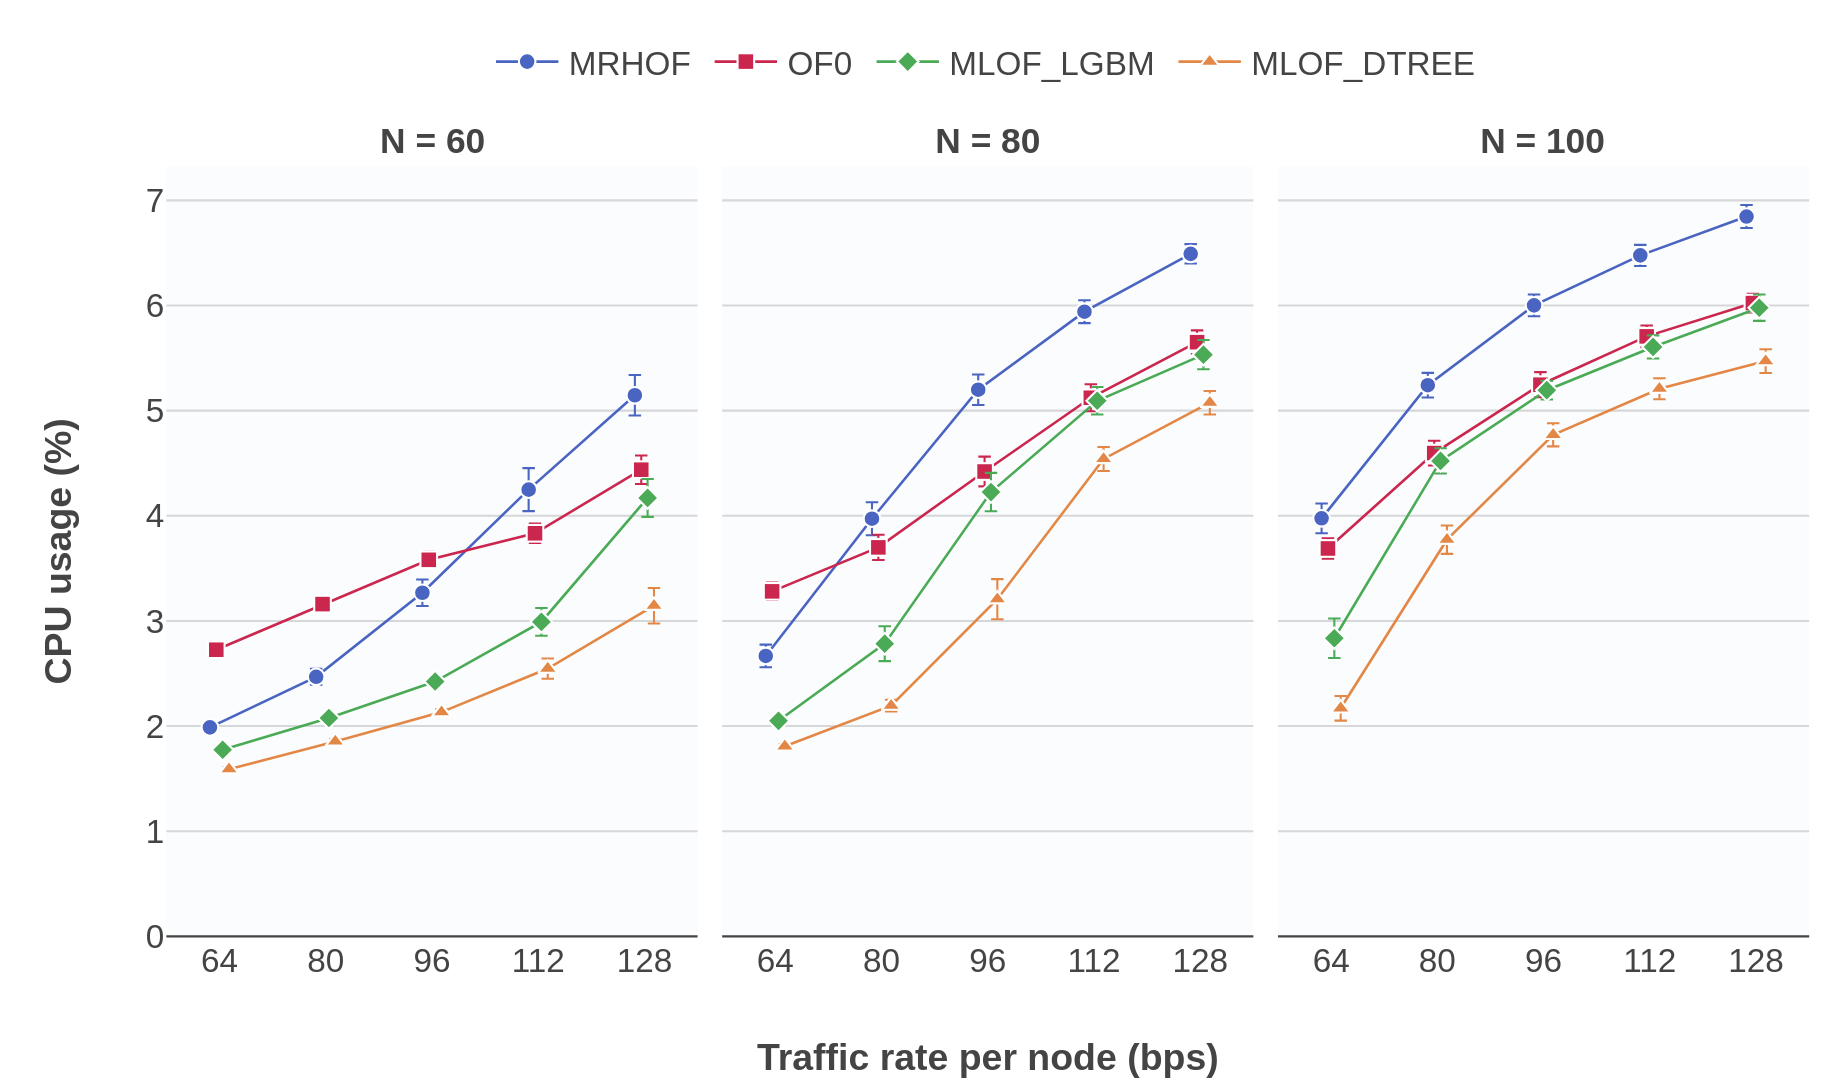
\includegraphics[width=1\textwidth]{assets/cpu_all_nodes.png}
        \caption{Average CPU usage with 95\% CI for 60, 80 and 100 nodes.}
        \label{fig:cpu_all_nodes}
    \end{center}
\end{fig}

\begin{fig}[tbh]
    \begin{center}
        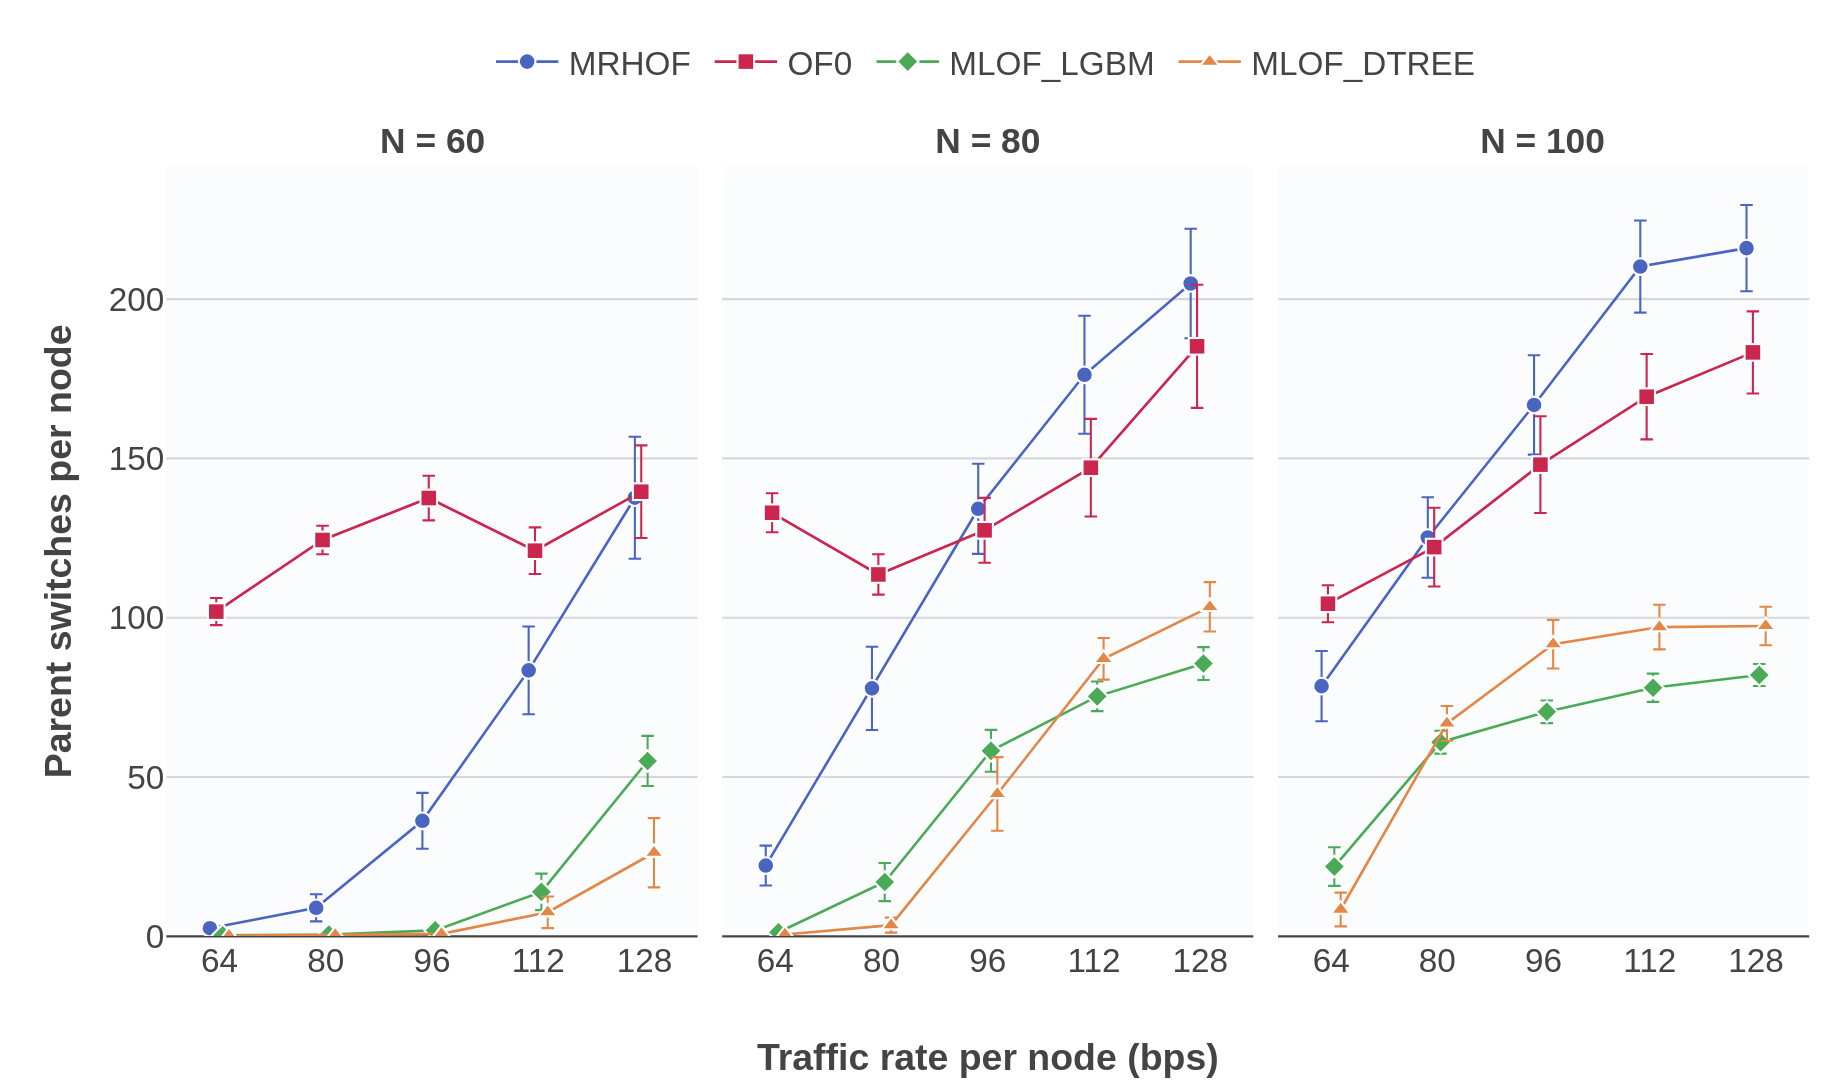
\includegraphics[width=1\textwidth]{assets/parent_switch_all_nodes.png}
        \caption{Average parent switches per node with 95\% CI for
        60, 80 and 100 nodes.}
        \label{fig:parent_switch_all_nodes}
    \end{center}
\end{fig}
% TODO: how to make these two figures go together
\begin{fig}[tbh]
    \begin{center}
        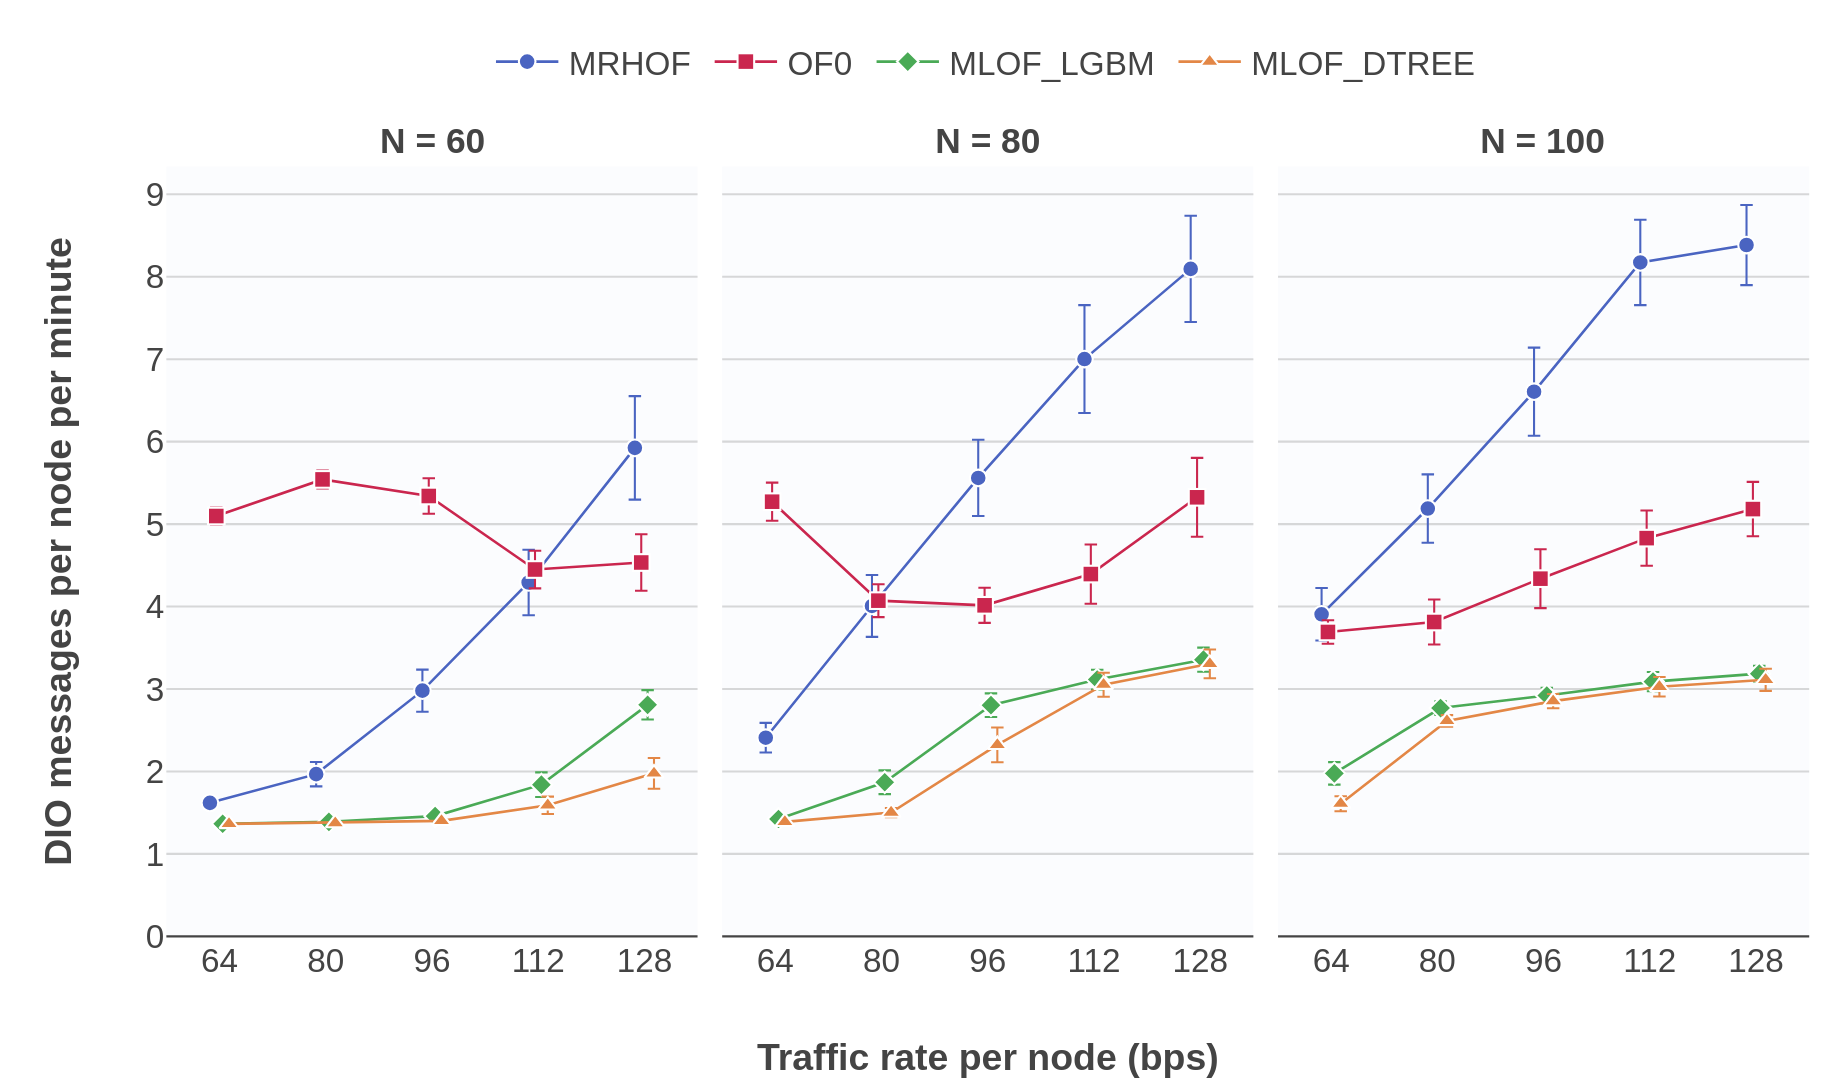
\includegraphics[width=1\textwidth]{assets/dio_sent_all_nodes.png}
        \caption{Average DIO messages sent per node per minute with
        95\% CI for 60, 80 and 100 nodes.}
        \label{fig:dio_sent_all_nodes}
    \end{center}
\end{fig}
% TODO: should I include more number for 80 and 100 nodes

Despite the additional computation required for model inference, both
MLOF variants use less CPU than the baseline OFs thanks to
more stable topology, fewer parent switches and DIO
transmissions, and lower average hop count.
\dtree{} achieves the lowest CPU usage in every configuration, 20\%
and 42\% below
MRHOF and OF0 at 60 nodes and 64~bps. The difference between
\dtree{} and \lgbm{} is most clearly attributable to the inference cost at
60 nodes and 64~bps, where both produce practically identical PDR, hop
count and DIO rates, yet \lgbm{} requires 1.78\% CPU compared with 1.59\%
for \dtree{}. This is consistent with the higher
computational complexity of the gradient-boosted ensemble discussed in
Section~\ref{sec:overhead}. At higher loads the gap widens, e.g.\ to
33\% at 128~bps, but here it also reflects the longer paths and more
frequent parent switches of \lgbm{}.

Since the evaluated topology does not use radio duty cycling, the
radio remains in receive mode and dominates the energy consumption of
each node. The reduction in CPU usage therefore translates to only a
modest saving in total energy. However, it indicates that the
inference overhead of MLOF is outweighed by the processing it saves,
and the benefit is expected to be more pronounced in duty-cycled
networks, where processing and transmissions account for a larger
share of the energy budget

\section{Overhead of MLOF}\label{sec:overhead}
\subsubsection{Model Inference Overhead}
On the Z1 platform, a single inference takes on average 13.0~$\mu$s
for \dtree{} and 118.8~$\mu$s for \lgbm{}. This may partly explain
why \lgbm{} performs worse than
\dtree{} in the network, even though the two models achieve similar
accuracy in the offline evaluation. Moreover, the inference overhead
grows with more frequent DIO messages and parent changes, which could
consume more share of the CPU compared. This may contribute to the
sharper degradation in the PDR as the load increases in both \dtree{}
and \lgbm{}.
% TODO: maybe packet loss during inference

\subsubsection{Memory Overhead}
As for the memory overhead, Table~\ref{tab:memory-overhead} shows the
ROM and RAM footprint of each OF. Compared with MRHOF, \dtree{}
requires about 4.3~kB more ROM on the server and 3.9~kB more on the
client, as well as 224 and 96 bytes more RAM, respectively. \lgbm{}
requires the same amount of RAM as \dtree{}, since both models are
stored as constants in ROM and the additional RAM is used only for the
shared metrics. However, \lgbm{} requires a further 2.9~kB of ROM
compared with \dtree{}, due to the larger gradient-boosted ensemble.
In all cases, the footprint remains well within the 92~kB of flash and
8~kB of RAM available on the Z1.

\begin{table}[h]
    \caption{Memory footprint of each objective function on the Z1 mote (in
    bytes), with \texttt{BUFFER\_SIZE}=8 and \texttt{NETWORK\_SIZE}=60.}
    \label{tab:memory-overhead}
    \begin{center}
        \begin{tabular}{lrrrr}
            \hline
            \textbf{OF} & \textbf{Server ROM} & \textbf{Server RAM} &
            \textbf{Client ROM} & \textbf{Client RAM} \\
            \hline
            OF0         & 42692 & 5752 & 44805 & 4886 \\
            MRHOF       & 42712 & 5752 & 44825 & 4886 \\
            \dtree{}  & 46978 & 5976 & 48745 & 4982 \\
            \lgbm{}   & 49858 & 5976 & 51625 & 4982 \\
            \hline
        \end{tabular}
    \end{center}
\end{table}

\subsubsection{DIO Overhead}
To share the load metrics between neighbours, MLOF appends a DAG
Metric Container option to every DIO message. The option consists of a
1-byte option type (\texttt{DAG\_METRIC\_CONTAINER}), a 1-byte option
length and a 1-byte container tag (\texttt{RPL\_DAG\_MC\_MLOF}),
followed by three metrics: the path CPU usage \texttt{path\_cpu}
(1~byte), the path packet rate \texttt{path\_ppm} (2~bytes) and the
hop count (1~byte). In total, each DIO carries 7 additional bytes
compared with OF0 and MRHOF.

MLOF of both models send fewer DIOs than the baseline OFs
thanks to a more stable topology, so that the share of the added
metrics remains lower. Over a one-hour simulation
of 60 nodes at 64~bps, \dtree{} sends about 4\,900 DIOs, totalling
408~kB (83~bytes each), compared with 443~kB for MRHOF and 1\,395~kB
for OF0 (76~bytes each).
At 100 nodes and 128~bps, \dtree{} sends 1\,550~kB of DIOs,
compared with 2\,363~kB for OF0 and 3\,824~kB for MRHOF. Combined
with the lower CPU usage and higher PDR reported above, this indicates
that the overhead introduced by MLOF is compensated by the
gains in routing stability.

\section{Routing Topology}
% TODO: probably can say that the model consider both hop count, path
% cpu and etx. Focusing on route with lower hop count and lower cpu,
% and with ext to avoid lossy link
